\section{Decomposition strategy} \label{benders}
\subsection{Benders reformulation}
As this above two-stage stochastic programming problem includes the complicating first-stage variables in the problem formulation, we can fix these variables and decompose the original large-scale problem into one master problem and $\lvert \omega \rvert$ subproblems (i.e. one subproblem for each scenario). Benders decomposition can be applied accordingly. Alternatively, the consensus ADMM can be implemented by relaxing the first-stage variables to be scenario-dependent. The original problem can be decomposed into $\lvert \omega \rvert$ subproblems as well, which nevertheless brings us $\lvert \omega \rvert-1$ complicating constraints. Therefore, implementing Benders decomposition is more favorable for this case.

In order to implement Benders decomposition, the real-time subproblems are re-formulated in their standard forms as below. The real-time power balance constraint is broken into two inequality constraints, such that we can guarantee the dual variables are non-negative.
This is due to the solver might give negative dual variables for inequality constraints. In this way, we can take absolute values of dual variables to guarantee the correctness of our algorithm.

\begin{equation}
    \forall s,
    \begin{cases}
\min  \sum_g  C_g^+ p_{g,s}^{+} - \sum_g  C_g^- p_{g,s}^{-} + C^{voll}\sum_d p_{d,s}^{shed} &\\
\textbf{S.t.} &\\
p_{g,s}^{+}-p_{g,s}^{-} \leq {P}_{g}^{max} - p_{g}^{\mathrm{DA}}: \quad \mu^1_{g,s} , \forall g &\\
-p_{g,s}^{+}+p_{g,s}^{-} \leq p_{g}^{\mathrm{DA}}: \quad \mu^2_{g,s} , \forall g  &\\
p_{w,s}^{spill} \leq p_{w,s}^{RT}:\quad \mu^3_{w,s}, \forall w &\\
p_{d,s}^{shed} \leq p_d^D:\quad \mu^4_{d,s},  \forall d &\\
\sum_{d \in \Psi_{n}} (- p_{d,s}^{shed})+\sum_{m \in \Omega_{n}} B_{n, m}\left(\theta_{n,s}^{RT}-\theta_{m,s}^{RT}\right)-\sum_{g \in \Psi_{n}} (p_{g,s}^{+}-p_{g,s}^{-}) \hspace{2cm} \\- \sum_{w \in \Psi_{n}} (-p_{w,s}^{spill}) \leq \sum_{m \in \Omega_{n}}B_{n, m}(\theta_{n}^{DA}-\theta_{m}^{DA}) + \sum_{w \in \Psi_{n}} (P_{w,s}^{RT}-P_w^{DA}) :\lambda_{n,s}^{RT1}, \forall n &\\
\sum_{d \in \Psi_{n}} (p_{d,s}^{shed})-\sum_{m \in \Omega_{n}} B_{n, m}\left(\theta_{n,s}^{RT}-\theta_{m,s}^{RT}\right)+\sum_{g \in \Psi_{n}} (p_{g,s}^{+}-p_{g,s}^{-}) \hspace{2cm} \\+ \sum_{w \in \Psi_{n}} (-p_{w,s}^{spill}) \leq- \sum_{m \in \Omega_{n}}B_{n, m}(\theta_{n}^{DA}-\theta_{m}^{DA}) -\sum_{w \in \Psi_{n}} (P_{w,s}^{RT}-P_w^{DA}) :\lambda_{n,s}^{RT2}, \forall n &\\
B_{n, m}\left(\theta_{n,s}^{RT}-\theta_{m,s}^{RT}\right) \leq F_{n,m}:\quad \eta^1_{n,m,s}, \forall n, \forall m &\\
-B_{n, m}\left(\theta_{n,s}^{RT}-\theta_{m,s}^{RT}\right) \leq F_{n,m}:\quad \eta^2_{n,m,s}, \forall n, \forall m &\\
p^{spill}_{w,s}\geq 0, \forall w &\\
p^{shed}_{d,s}\geq 0, \forall d &\\
p_{g,s}^+, p_{g,s}^- \geq 0, \forall g &\\
\theta^{RT}_{(n=r e f),s}=0 &\\
     \end{cases}  
\end{equation}



Following this, one can write the master problem for Benders decomposition as below, where (\ref{cut}) is the optimality cut. In this sense, multi-cut technique is used for generally faster convergence. The convergence criteria is bound gap less than $10^{-6}$.

\begin{subequations}
\begin{equation} \label{bendersobj}
    \underset{p_g^{DA(i)}, P_w^{DA(i)}, \theta_n^{DA(i)}}{\min} \sum_g C_g P_g^{DA(i)} + \sum_s \Phi_s \alpha_s^{(i)}
\end{equation}
\begin{equation}
    \alpha_s^{(i)} \geq \alpha^{down}, \forall s
\end{equation}
\centerline{(\ref{2.production}) - (\ref{2.ref})}
\begin{equation} \label{cut}
\begin{split}
    \alpha_s^{(i)} \geq  -\sum_g\mu^{1(i-1)}_{g,s}({P}_{g}^{max} - p_{g}^{\mathrm{DA{(i)}}}) - \sum_g\mu^{2(i-1)}_{g,s}p_{g}^{\mathrm{DA{(i)}}}-\sum_w\mu^{3(i-1)}_{w,s}p_{w,s}^{RT} -  \sum_d\mu^{4(i-1)}_{d,s}p_d^D \\- \sum_n \lambda_{n,s}^{RT1(i-1)} \left ( \sum_{m \in \Omega_{n}}B_{n, m}(\theta_{n}^{DA{(i)}}-\theta_{m}^{DA{(i)}}) + \sum_{w \in \Psi_{n}} (P_{w,s}^{RT}-P_w^{DA{(i)}})  \right)\\
    - \sum_n \lambda_{n,s}^{RT2(i-1)} \left ( -\sum_{m \in \Omega_{n}}B_{n, m}(\theta_{n}^{DA{(i)}}-\theta_{m}^{DA{(i)}}) - \sum_{w \in \Psi_{n}} (P_{w,s}^{RT}-P_w^{DA{(i)}})  \right)\\-\sum_{n,m}\eta^{1(i-1)}_{n,m,s}F_{n,m}-\sum_{n,m}\eta^{2(i-1)}_{n,m,s}F_{n,m}, \forall s
    \end{split}
\end{equation}
\end{subequations}

% \subsection{Case study}
% The algorithm terminates after cycles. The lower and upper bound are depicted in fig.\ref{fig:bound}.
% \begin{figure}[h]
%     \centering
%     \includegraphics{}
%     \caption{Lower and upper bound for Benders decomposition}
%     \label{fig:bound}
% \end{figure}

The general steps for running Benders decomposition includes:
\begin{enumerate}
    \item Run master problem, update lower bound, which is objective of master problem;
    \item Derive first-stage variables, run subproblems and update upper bound which can be computed with $\sum_g C_gP_g^{DA}+\sum_s \Phi_s g(s)$ with g(s) the objective of subproblems;
    \item Compare upper bound and lower bound to determine if the problem converges;
    \item If converged, terminate and output;
    \item Otherwise add optimality cuts into the master and go to step 1.
\end{enumerate}

\subsection{Case study}
In this case, we test the Benders decomposition by comparing it to the direct solution. The algorithms converge after around 7-9 cycles and reach the same result as direct solution. The lower bounds and upper bounds updates are shown in fig. \ref{fig:mean and std of nets}. The computation time is reported in tab. \ref{benders}. In our case, we can obtain direct solution with Gurobi solver very quickly. Benders decomposition on the other side, takes much more time. However, as the problem complexity increases, such as we introduce integer variables in the first stage problem, Benders decomposition would be more useful.

    \begin{figure*}
        \centering
        \begin{subfigure}[b]{0.475\textwidth}
            \centering
            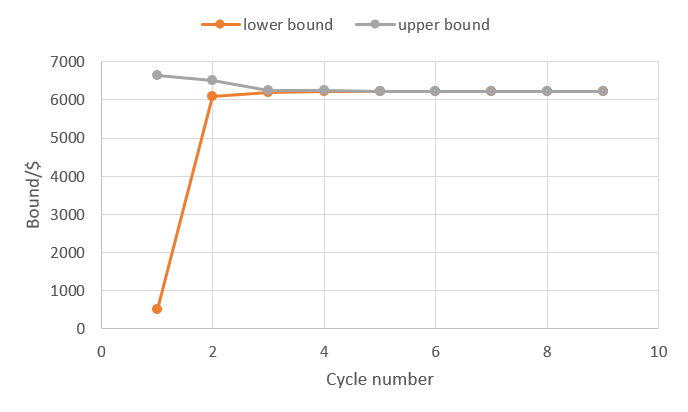
\includegraphics[width=\textwidth]{figures/BOUND5.png}
            \caption[Network2]%
            {{\small 5 scenarios}}    
            \label{fig:mean and std of net14}
        \end{subfigure}
        \hfill
        \begin{subfigure}[b]{0.475\textwidth}  
            \centering 
            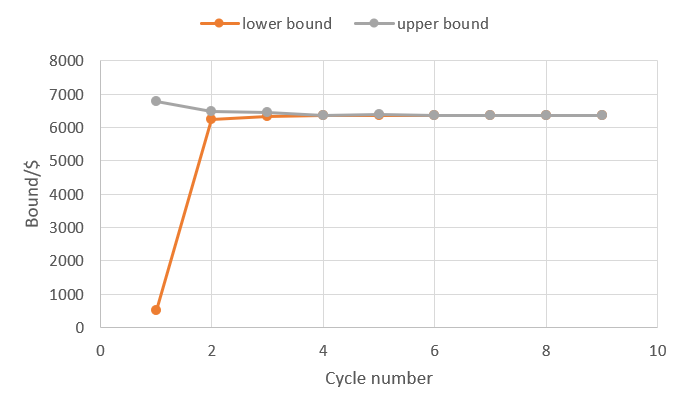
\includegraphics[width=\textwidth]{figures/BOUND10.png}
            \caption[]%
            {{\small 10 scenarios}}    
            \label{fig:mean and std of net24}
        \end{subfigure}
        \vskip\baselineskip
        \begin{subfigure}[b]{0.475\textwidth}   
            \centering 
            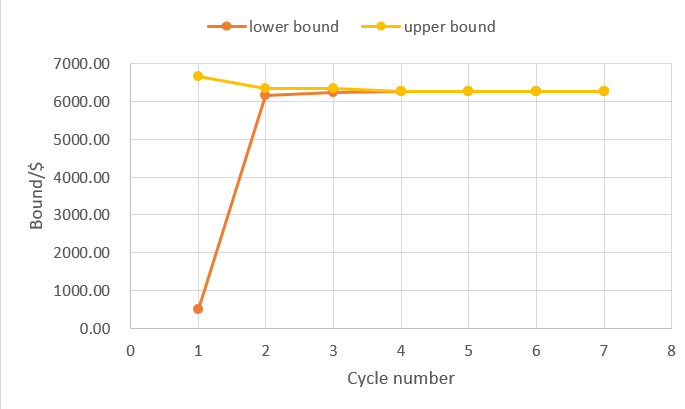
\includegraphics[width=\textwidth]{figures/BOUND20.png}
            \caption[]%
            {{\small 20 sceanrios}}    
            \label{fig:mean and std of net34}
        \end{subfigure}
        \quad
        \begin{subfigure}[b]{0.475\textwidth}   
            \centering 
            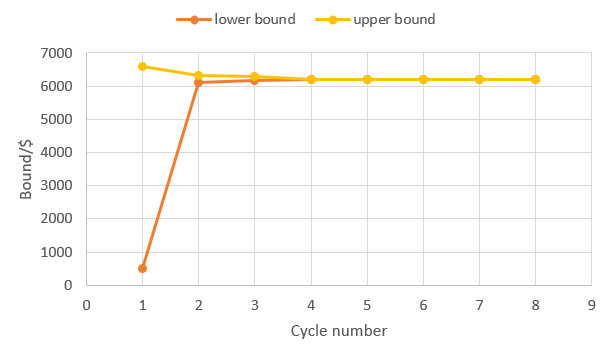
\includegraphics[width=\textwidth]{figures/BOUND30.png}
            \caption[]%
            {{\small 30 scenarios}}    
            \label{fig:mean and std of net44}
        \end{subfigure}
        \caption[]
        {\small Lower and upper bound update in Benders decomposition with different number of scenarios} 
        \label{fig:mean and std of nets}
    \end{figure*}

\begin{table}[h]
    \centering
    \begin{tabular}{|c|c|c|}
    \hline
     \textbf{Scenario number}    & \textbf{Direct} & \textbf{Benders} \\
         \hline
       5  & 0.94 s  & 14.59 s\\
       \hline
       10 & 1.73 s& 29.71 s\\
       \hline
       20 & 2.07 s & 26.04 s\\
         \hline
         30 & 2.05 s & 44.90 s\\
         \hline
    \end{tabular}
    \caption{Computation time for direct solution and Benders decomposition}
    \label{tab:benders}
\end{table}